\documentclass[cic,tc,english]{iiufrgs}

\usepackage[utf8]{inputenc}   % pacote para acentuação
\usepackage{graphicx}         % pacote para importar figuras
\graphicspath{{../images/}}
\usepackage{array}
\newcolumntype{L}[1]{>{\raggedright\let\newline\\\arraybackslash\hspace{0pt}}m{#1}}
\usepackage{times}            % pacote para usar fonte Adobe Times
% \usepackage{palatino}
% \usepackage{mathptmx}       % p/ usar fonte Adobe Times nas fórmulas
\usepackage[alf,abnt-emphasize=bf]{abntex2cite}	% pacote para usar citações abnt
\usepackage{cite}
\usepackage{subfig}
\usepackage{caption}
\newcommand \eg {{\it e.g.}}
\newcommand \ie {{\it i.e.}}
\newcommand \red[1] {\textcolor{red}{#1}}

\title{A Converter for Physically-Based Renderer Scenes}
\author{Hagemann}{Luiza de Azambuja}
\advisor[Prof.~Dr.]{Neto}{Manuel Menezes de Oliveira}

\keyword{physically-based rendering}
\keyword{scene conversion}
\keyword{PBRT}
\keyword{Mitsuba}
\keyword{LuxRender}

\begin{document}

\maketitle

% dedicatoria
% \clearpage
% \begin{flushright}
%     \mbox{}\vfill
%     {\sffamily\itshape
%       ``If I have seen farther than others,\\
%       it is because I stood on the shoulders of giants.''\\}
%     --- \textsc{Sir~Isaac Newton}
% \end{flushright}

% agradecimentos
%\chapter*{Acknowledgements}


% resumo na língua do documento
\begin{abstract}
    Physically-based rendering systems use proprietary scene description formats. Thus, by selecting a given renderer for the development of a new technique, one is often constrained to test and demonstrate it on the limited set of test scenes available for that particular renderer. This makes it difficult to compare techniques implemented on different rendering systems. 
We present a system for automatic conversion among scene description formats used by physically-based rendering systems. 
It enables algorithms implemented on different renderers to be tested on the same scene, providing better means of assessing their strengths and limitations. 
Our system can be integrated with existing development and benchmarking APIs, lending to full orthogonality among algorithms, rendering systems, and scene files.
\end{abstract}

% resumo na outra língua
% como parametros devem ser passados o titulo e as palavras-chave na outra língua, separadas por vírgulas
\begin{englishabstract}
    Placeholder.
\end{englishabstract}{physically-based rendering, meta-research, PBRT, mitsuba, luxrender}

% lista de figuras
\listoffigures

% lista de tabelas
% \listoftables

% lista de abreviaturas e siglas
\begin{listofabbrv}{PBR}
    \item[PBR] Physically Based Rendering
    \item[MC] Monte Carlo
\end{listofabbrv}

% idem para a lista de símbolos
% \begin{listofsymbols}{$\alpha\beta\pi\omega$}
%     \item[$\sum{\frac{a}{b}}$] Somatório do produtório
%     \item[$\alpha\beta\pi\omega$] Fator de inconstância do resultado
% \end{listofsymbols}

% sumario
\tableofcontents

% capitulos
\section{Introduction}
\label{sec:introduction}

Monte Carlo ray tracing is currently the only practical solution for simulating global illumination effects in complex environments.
Due to its high computational cost, several techniques have been introduced to reduce rendering time through improved sampling~\cite{Heck2013, Pilleboue:2015} and reconstruction strategies~\cite{Sen2012, Rousselle2013, Kalantari2015, Bitterli2016}. When developing such new techniques, researchers often implement them on top of existing rendering systems as a way of leveraging available infrastructure to perform functions (\eg, ray-traversal acceleration, ray-primitive intersections, etc.) that are orthogonal to the proposed methods.

Unfortunately, the various rendering systems use proprietary scene description formats. While modeling visually-pleasing scenes requires significant artistic skills, manual conversion between proprietary formats requires knowledge of the specific formats and tend to be extremely time consuming (up to several days per scene~\cite{tungsten}). 
Thus, by selecting a given rendering system one is often constrained to test and demonstrate the proposed techniques on the limited set of test scenes available for that renderer. This apparently simple limitation has profound implications, as it constrains a direct comparison between Monte Carlo (MC) rendering techniques that have been implemented using different rendering systems. In this case, one often has to compare the quality of algorithms using disjoint sets of scenes, which, is not the ideal case.    
    
We present {\it a system for automatic conversion among scene file formats used by Monte Carlo physically-based rendering systems}. 
Our solution significantly expands the repertoire of scenes available for testing, validation, and benchmarking of MC rendering algorithms.  
Currently, our system handles conversions among PBRT v3~\cite{PBRT:v3}, Mitsuba~\cite{mitsuba}, and LuxRender~\cite{luxrender}, which are three of the most popular physically-based renderers (PBR). Extending it to support additional renderes is straightforward. Our solution (discussed in Section~\ref{sec:systemarch}) consists of {\it importing} any source scene description into a canonical representation, which can then be {\it exported} to other scene formats. 
%By specializing the import and export classes to the various formats, our system can convert among arbitrary scene file formats.     
%
Figure~\ref{fig:teaser} illustrates the use of our system to perform automatic conversion of a scene represented in the PBRT v3 format. 
%The image shown on the left is the PBRT v3 rendering. 
The images at the center and on the right show, respectively, the renderings produced by Mitsuba and by LuxRender, from converted scenes files. Note the correct representation of the 
%scene elements that include multiple 
various materials (glass, plastic, and metal).

Our work does not introduce a new physically-based rendering technique per se. Instead, it falls in the area of {\it meta-research} systems, which are systems designed to facilitate and improve the research process. Meta-research systems are quite common in computer graphics~\cite{Santos:2018:FBKSD, Ragan-Kelley2012,Buck2004,Mark2003} and computer vision~\cite{MiddleburyStereo, MiddleburyFlow, AlphaMatting, VideoMatting}, where they have led to significant progress in these fields. 
%In a work particularly relevant to us,  
Recently, Santos et al.~\cite{Santos:2018:FBKSD} introduced a framework for developing and benchmarking MC sampling and denoising algorithms. This is achieved by providing an API the decouples the developed techniques from the used rendering system. While it allows a technique to be tested on any rendering system that supports the proposed API, each rendering system is still constrained to a limited set of test scenes. Our system is orthogonal to and complements the API described in~\cite{Santos:2018:FBKSD}, lending to full orthogonality, among algorithms, rendering systems, and scene files.
%by allowing an MC technique to be tested on any combination of rendering systems and scene files. 
%The system is also available for download~\cite{sceneConverter}.    

The {\bf contributions} of our work include:
\begin{itemize}
	\item A system for automatic conversion among scene file formats used by Monte Carlo physically-based rendering systems (Section~\ref{sec:systemarch}).
	It enables algorithms implemented on different rendering systems to be tested on similar scene descriptions, giving developers and end users a better assessment of the strengths and limitations of MC rendering techniques;
	\item A mechanism for achieving full orthogonality among MC rendering algorithms, rendering systems, and scene files (Section~\ref{sec:systemarch}). This is achieved in combination with the API provided in~\cite{Santos:2018:FBKSD}. 
\end{itemize}

%
%Ever since the development of modern Computer Graphics, one of the goals 
%researchers aspired to was being able to synthesize images indistinguishable 
%from real photographs. In order to produce physically accurate images, the 
%process of image synthesis - also called \textbf{rendering} - simmulates the 
%interaction of light with the representation of a three-dimensional scene. 
%
%\textbf{Physically-Based Rendering (PBR)} is a complex process that requires 
%thorough knowledge of optics, material properties, geometry and light 
%propagation.
%
%\subsection{Physically Based Rendering (PBR)}
%Over the years, PBR became quite popular and was widely incorporated into the 
%entertainment industries. From movies to videogames, from ads to interior 
%design, PBR made it possible for artists to bring their creations and their 
%vision one step closer to reality. Today, we can say that many - if not most - 
%algorithms used in computer animation, geometric modeling and texturing require 
%that their results be passed through some sort of rendering process.
%
%As PBR popularity grew, a brand new market opened up for physically-based (PB) 
%renderers. Following the creation of \textit{PBRT} \cite{pbrt} and the publishing of 
%\textit{"Physically Based Rendering: From Theory to Implementation"} 
%\cite{pbrtBook}, several other research-oriented renderers were created. Among them 
%is \textit{Mitsuba} \cite{mitsuba}, one of the renderers chosen for this research, which places 
%strong emphasis on experimental rendering techniques.
%
%Following the lead of Pixar's \textit{Renderman}, many 
%commercial and performance-oriented renderers appeared on the market. Focused on 
%animation techniques and visual effects for movies, these renderers provide 
%well-established, stable rendering techniques. These renderers, such as 
%\textit{LuxRender} \cite{luxrender} and \textit{Octane}, are 
%state-of-the-art renderers used by the animation and gaming industries.
%%https://www.blenderguru.com/articles/render-engine-comparison-cycles-vs-giants
%
%Even with different applications, the vast majority of modern PB renderers 
%follows the same general guidelines for defining scene directives and world 
%descriptions. Scene directives establish parameters such as which integration 
%and sampling techniques the renderer must use, the view matrix and other camera 
%properties. World descriptions state which objects compose the scene and which 
%materials must be used to render them. This ensemble of descriptions is what, in 
%PBR, is called a \textbf{scene}.
%
%\subsection{Rendering a Scene}
%% - the scene
%Starting with \textit{PBRT}, most PB renderers have used a similar, traditional​ 
%structure to describe scenes.
%
%These scenes are usually created by a 3D artist, who will use a modeling 
%software (such as Blender, 3D Max or Maya) to draw the objects, choose their 
%materials and then create the object files. These files will then be instanced 
%in the scene file and interpreted by the renderer.
%
%% - stating the problem/motivation: making scenes is hard 
%% (reference: http://www.laubwerk.com/home/)
%But even with an artist’s expertise, creating scenes is still a complex process. 
%For instance, scenes created for building overviews and interior design often 
%compile hundreds of 3D models and dozens of customized materials and textures. Each material and texture 
%has to be carefully defined, taking into account the renderer's limitations and 
%particularities.
%
%After a scene is created and rendered, all the hard work invested by the artist 
%is stored, waiting for a possible future use. However, should the artist choose 
%to change renderers, the scene file they created so diligently would have to be 
%rewritten and/or heavily modified.
%
%Converting a scene file from one renderer format to another is very difficult 
%and time consuming. Aside from adapting material and light properties - which 
%can be hard since sometimes renderers don't provide the same features -, the 3D 
%object formats supported may not be the same. For instance, \textit{Mitsuba} 
%supports the Object File Wavefront 3D (.obj) format while \textit{PBRT} does 
%not.

%Creating free resources in order to help rendering research, Benedikt Bitterli 
%\cite{resources16} manually converted 32 scenes for his renderer \textit{Tungsten} 
%\cite{tungsten}, later converting them to \textit{PBRT} and \textit{Mitsuba}. 
%According to him, \textit{"this process is time intensive (up to several days 
%per scene)"}.
\chapter{Related Work}
\label{sec:related_work}

In this chapter we discuss relevant, similar systems developed as meta-reseach, such as other attempts to convert scenes and exporting a generic 
scene format into different renderer-specific outputs. This chapter is meant to contextualize the reader in the state-of-the-art in converting PBR scene files.

\section{Similar Conversion Tools}

With the addition of new physically-based renderers to the market, the number of incompatible file formats began to grow. There were a few initiatives to solve this problem, the greatest one being the proposal of a common file format.

Back in 2004, Arnaud and Barnes created COLLADA \cite{collada}, a XML schema file format that intended to unify representation of digital assets among 
various graphics software applications. Ever since it became property of the Khronos Group, several companies included a COLLADA module on their 3D modeling 
softwares or game engines. However, there were few physically-based renderers that adhered to this file format, one of the few being Mitsuba. That might have 
happened because COLLADA files only include information about the geometry present in the scene - they don't store any information about other rendering 
options, such as camera positioning or integration techniques.

To the best of our knowledge, no previous system has performed automatic scene conversion among the major MC rendering systems. Bitterli has converted 32 scenes of various complexities and origins from Tungsten to PBRT v3 and Mitsuba using some scripts~\cite{tungsten}. These scripts, however, are specific for conversions from Tungsten to these two renderers and are not publicly available.

RenderToolbox3 is a MATLAB tool developed for assisting vision research~\cite{rendertoolbox}. It imports a scene containing geometric objects described as COLLADA XML files, and allows one to associate to them reflectance measurements from a MATLAB Psycophysics Toolbox~\cite{Brainard1997}. Such reflectance measurements are converted to multispectral reflectance representations compatible to PBRT and Mitsuba. A script then renders the objects with the associated multispectral representations using PBRT or Mitsuba. RenderToolbox3 is a visualization tool for exploring the impact of different reflectance and illuminating properties on human perception.

\cite{rendertoolbox} is a system that imports COLLADA XML files into a MATLAB system and uses different rendering techniques in order images as close to 
reality as possible. Their system uses integrated PBRT and Mitsuba rendering is capable of storing their data structure into their respective scene file 
formats. The system does not convert scene files among rendering systems. 

\section{Meta-Research Systems in Computer Graphics}

Several systems have been developed to support research in computer graphics. Some well-known examples include Cg~\cite{Mark2003}, Brook~\cite{Buck2004}, and Halide~\cite{Ragan-Kelley2012}.

Cg is a general-purpose programming language designed to support the development of efficient GPU applications, and has stimulated a lot of research efforts in shader-based rendering techniques~\cite{Policarpo2005, Policarpo2006, Wyman2005, Oliveira2007RRT}.  

Brook~\cite{Buck2004} is system for general-purpose computation that allows one to exploit the inherent parallelism of modern GPUs without having to deal with GPU architecture details. These kinds of systems were an inspiration that led to the development of CUDA~\cite{Nickolls2008}.

Halide~\cite{Ragan-Kelley2012} is a system designed to optimize image-processing applications on multiple hardware platforms by separating the algorithm description from its schedule. The system has been recently extended to support differentiable programming for image processing and deep learning~\cite{Li2018-Halide-Diff_Prog}. 

All these systems focus on generating efficient code while freeing the user from GPU architectural details. All goal, in turn, is to make high-quality scenes availability independent of one's choice of rendering system. 

Santos et al. have recently presented a framework for developing and benchmarking MC sampling and denoising algorithms. They use an API to decouple algorithms from rendering systems, allowing for the same algorithm to be tested on multiple rendering systems. By doing so, they also increase the set of scenes an algorithm can be tested with. However, in order to use a given test scene, the rendering system for which the scene was created would have to be used as well. 


\chapter{Review of Global Illumination and MC Ray Tracing}
%\chapter{Theoretical Foundations}
\label{sec:theory}

This chapter reviews important concepts about  global illumination techniques such as \textit{Ray Tracing}, followed by 
a description of 
%important explanations about 
the techniques implemented by the renderers used in our work (MC Ray Tracing). We do not delve too deep in the implementations of the techniques discussed in this chapter --- we provide a general understanding of the process in order to better situate the reader.

\section{Global Illumination Algorithms}

Global illumination algorithms try to synthesize realistic pictures by
%have as their goal add more realistic lighting to 3D scenes, 
taking into account both direct and indirect illumination, at the expense of a higher computational cost when compared to local illumination techniques. 
%the Light Transport around the scene, and not only the light coming directly from the light source. 
%Images rendered using these algorithms are more photorealistic than images rendered using direct illumination algorithms at the expense of a higher computational cost. 

{\it Light transport} models the interaction between light and the surface in the scene, 
%using the principle that 
where some fraction of the light incident to a surface is reflected back to the environment. Modeling this reflection requires its spectral and directional distributions, which differ depending on the material properties of the surface. Earlier algorithms modeled these materials as ideal diffuse (Lambertian surfaces) and ideal specular (mirrors) for simplicity.

Starting at a light source (L), a light ray may bounce several times at specular (S) and diffuse (D) surfaces before reaching the eye (E). These interactions can be represented using regular expressions such as L(S|D)*E. Rendering algorithms can be caracterized by the kinds of paths they support.

Local illumination models, such as the Phong lighting model, 
%Gouraud Shading or Phong Shading, 
have the light hit the scene once before reaching the eye (LDE or LSE). Algorithms that have a good representation of specular reflection, such as Ray Tracing~\cite{Whitted:1980}, perform at most one bounce on diffuse surfaces and can perform any number of bounces on specular surfaces (LDS*E or LS*E).

\section{Ray Tracing}

\textit{Ray Tracing} \cite{Whitted:1980} is a global illumination algorithm that handles multiple inter-reflections among shiny surfaces, producing 
high-quality results for shiny surfaces. In Ray Tracing, we trace rays from the eye through each pixel of the image, searching for the closest intersected object along each ray. When an intersecting surface is found, the algorithm shoots a shadow ray to determine whether this surface is hidden from the light source and locally evaluates an illumination function. The incoming ray is then either reflected or refracted (in other words, \textit{bounced}), repeating the process until 
%the original ray reaches 
a certain amount of bounces is achieved, the contributions of subsequent hits become negligible, or the ray does not intersect any other object in the scene. This process is illustrated in Figure \ref{fig:raytracing}.

\begin{figure}[h]
  \centering
  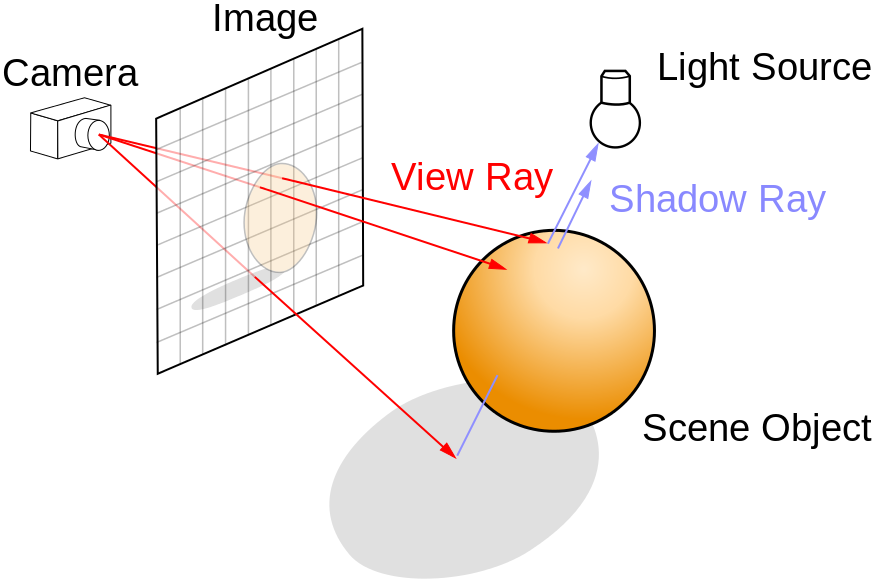
\includegraphics[width=0.45\textwidth,height=\textheight,keepaspectratio]{images/3_theoretical_foundations/raytracing.png}
  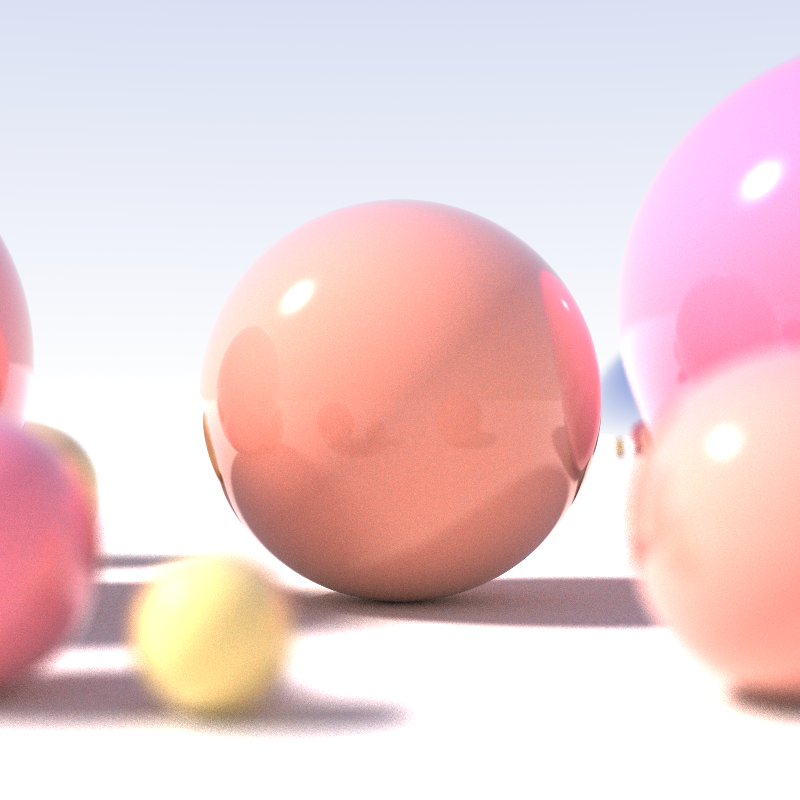
\includegraphics[width=0.45\textwidth,height=\textheight,keepaspectratio]{images/3_theoretical_foundations/raytracingexample.png}
  \caption{Visual illustration of the Ray Tracing algorithm (left) and an example of a scene rendered with the algorithm (right), extracted from \cite{wiki:raytracing}}
  \label{fig:raytracing}
\end{figure}

% While it may seem strange to send rays away from the camera - which is the opposite of how photographs are generated -, it is more cost-efficient as most light rays that incide on the scene do not reach the camera. Computing light paths is a strenuous task, and cutting back on this task load shortens the rendering time considerably.

Because a Lambertian surface reflects rays in all directions, there is a very-high computational cost associated with calculating reflections in diffuse surfaces. In order to reduce this cost, Ray Tracing algorithm approximates the actual diffuse reflection (using Phong's illumination model, for instance), thus not representing it with as much realism as a specular surface.

True realism can only be achieved when an algorithm approximates the \textit{Rendering Equation} \cite{Kajiya:1986} - which describes the full light transport.
%every physical effect of light flow. 
This method will be further discussed in our next section. 

\section{The Rendering Equation}

An important concept for global illumination algorithms is that of \textit{radiance}, which describes how much power arrives at (or leaves from) a certain point on a surface per unit solid angle and per unit projected area. Radiance can be thought of as the number of photons arriving per time at a small area from a given direction, and it describes the intensity of light at a given point in space in a given direction. Radiance remains constant along the light rays passing through empty space, and when computed, it captures the appearance of objects in the scene.

Another important concept is that of the \textit{Bidirectional Reflectance Distribution Function} (BRDF), a function that describes the local illumination model of a given material. The BRDF can be perceived as a constant of proportionality between the amount of incident light and the reflected light along a direction. Using the BRDF, we are able calculate the total amount of light reflected by a surface with a given material in a specific direction as an hemispherical integral over all possible incident directions, as seen in Figure \ref{fig:brdf}.

\begin{figure}[h]
  \centering
  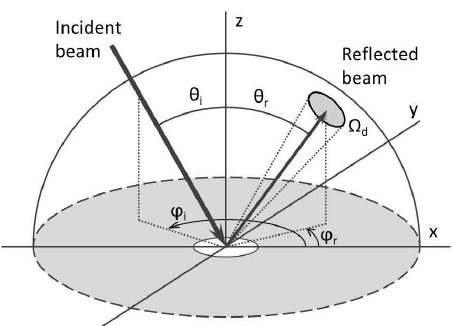
\includegraphics[width=0.5\textwidth,height=\textheight,keepaspectratio]{images/3_theoretical_foundations/brdf.png}
  \caption{Example of how BRDF describes a local illumination model for a surface, extracted from \cite{brdf}}
  \label{fig:brdf}
\end{figure}


These concepts and properties were used in the \textit{Rendering Equation} \cite{Kajiya:1986}, which models the global light transport in a scene. Modeling global illumination means that one would need to consider the light path across the entire scene, not only one interaction - which was the main problem with techniques such as Ray Tracing. 

The Rendering Equation is described as:

% $$L_o (x \rightarrow \omega) = L_e (x \rightarrow \omega) + \int_{\Omega} f_r (x, s \rightarrow \omega) L_i (x \leftarrow s) V(x, x') G(x, x') ds $$
$$ L_o (x, \omega_o) = L_e (x, \omega_o) + \int_{\Omega} f_r (x, \omega_i, \omega_o) L_i (x, \omega_i) (\omega_i \cdot n) d\omega_i $$

We can interpret this equation as: the total radiance $L_o$ directed outward from point $x$ along direction $\omega_o$ is composed of the radiance emitted ($L_e$) from point $x$ along direction $\omega_o$ and the sum of the radiance $L_i$ directed inward toward $x$ coming from every possible direction $\omega_i$ in hemisphere $\Omega$. $L_i$ is affected by the surface's BRDF ($f_r$), which dictates the proportion of light that is reflected from $\omega_i$ to $\omega_o$, and by the weakening factor $\omega_i \cdot n$ caused by $\omega_i$'s incident angle. 

The Rendering Equation cannot be directly evaluated, as radiance (L) is present in both sides of the equation; it is impractical to solve with traditional quadrature methods. However, this equation \textit{can} be evaluated by \textit{Monte Carlo Integration}, the technique used in \textit{Monte Carlo Ray Tracing}.

\subsection{Monte Carlo Ray Tracing}

Monte Carlo Integration (MCI) is a technique that uses statistical principles to estimate complicated integrals. It assumes that if a $x$ is a random variable, then $f(x)$ is also a random variable that can be characterized by its probability distribution. We can approximate $f(x)$ with n random samples along $f(x)$'s probability distribution $p(x)$. The MC estimator of an arbitrary function $g(x)$ can be expressed as:

$$ \int g(x)dx \approx \frac{1}{n} \sum_{i = 1}^{n} \frac{g(X_i)}{p(X_i)}$$

The convergence rate for MCI is $O(\frac{1}{\sqrt{n}})$ regardless of the smoothness of the integrand at any dimension. The technique requires only sampling and point evaluation and can be used to solve a vast array of problems. It does, however, have a high variance that can, in the case of MC rendering, appear as noise. In order to reduce the variance naturally produce by this method, one must greatly increase the number of samples.

The concept of \textit{Importance Sampling} was created to reduce this high variance, exploiting the fact that the MC estimator converges faster if the points are sampled from a distribution $p(x)$ that is similar to $f(x)$. This process is illustrated in Figure \ref{fig:importance}

\begin{figure}[h]
  \centering
  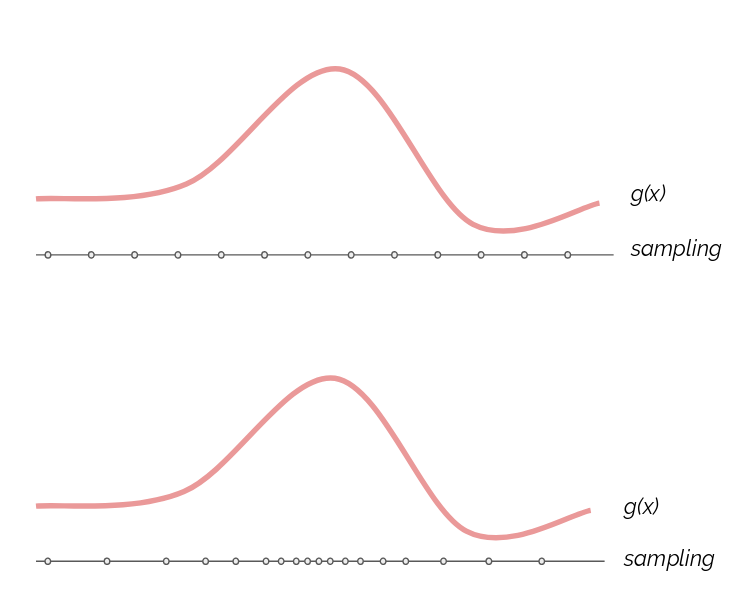
\includegraphics[width=0.5\textwidth,height=\textheight,keepaspectratio]{images/3_theoretical_foundations/importances.png}
  \caption{Illustration of how uniform sampling (top) and how importance sampling (bottom) sample $g(x)$}
  \label{fig:importance}
\end{figure}

MC Ray Tracing, commonly called \textit{Path Tracing}, uses MCI to approximate the Rendering Equation, estimating the radiance for each point and produce photorealistic images. It is able to naturally reproduce very complicated effects such as motion blur (sampling over time) and depth-of-field (sampling through a lens). However, MC Ray Tracing has a very high computational cost - even using Importance Sampling, the number of samples required to render a large scene is in the order of thousands per pixel. Generating these images can take up to hours depending on the complexity of the scene. 

Notwithstanding, MC Ray Tracing is currently the only practical solution for simulating global illumination effects in complex environments. It is implemented in virtually every modern physically-based renderer, featuring several other algorithms using MCI, such as Photon Mapping and Metropolis Light Transport.
\chapter{Automatic Scene Conversion} 
\label{sec:systemarch}

Our system consists of two main components: an {\it import module} that reads an arbitrary scene file format and generates an equivalent description in a {\it canonical} scene representation; and an {\it export module} that takes our canonical representation and exports it to a target rendering system file format. The complete process is illustrated in Figure \ref{fig:sysarch}. 
Currently, our system supports \textit{PBRT v-3}~\cite{PBRT:v3}, \textit{Mitsuba}~\cite{mitsuba}, and \textit{LuxRender}~\cite{luxrender}, as these are three of the most popular rendering systems.
This architecture, however, is quite flexible. Supporting additional rendering systems only requires specializing the import and export methods to handle the new formats. 
%Moreover, it can be easily integrated with the API described in~\cite{Santos:2018:FBKSD}.   
%
Next, we describe the main components of our system.

%Our Proof of Concept (PoC) encompassed \textit{PBRT} \cite{pbrt}, \textit{Mitsuba}
%\cite{mitsuba} and \textit{LuxRender} \cite{luxrender}, as these are three of
%the most popularly used renderers in the community. This architecture, however,
%is easily extensible: adding other renderers would be a simple task of writing
%an import and a conversion module.



%converting pipeline is subdivided into three main states: the \textbf{Import
%Module}, the \textbf{Canonical Scene Representation} and the \textbf{Conversion
%Module}, as illustrated in Figure \ref{fig:sysarch}. Given an arbitrary input
%file format, our converter is able to import the scene and transform it into a
%generic, canonical representation and then export it to different output
%formats.

\begin{figure}[h]
  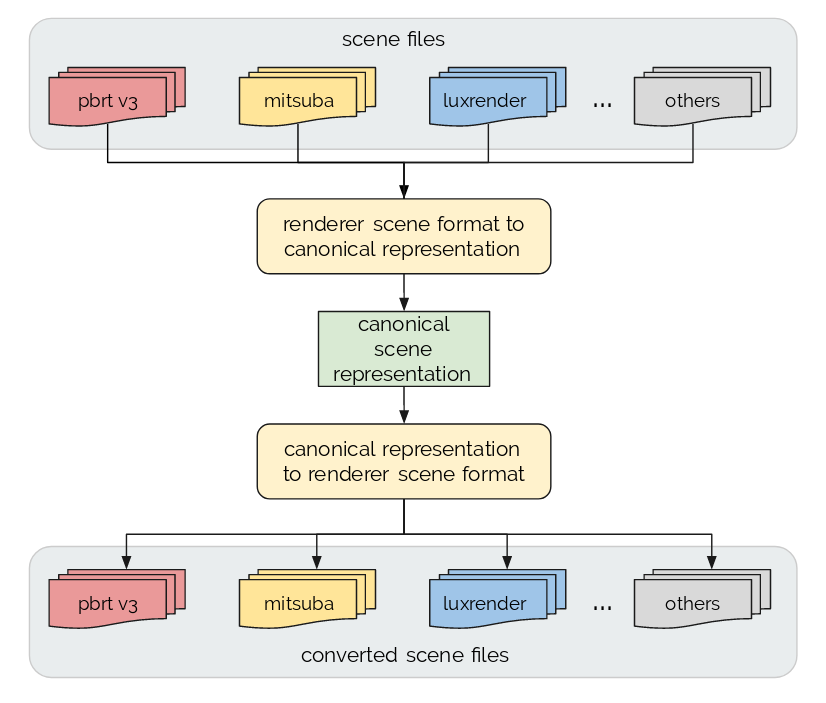
\includegraphics[width=\textwidth,height=\textheight,keepaspectratio]{images/4_system_architecture/architecture.png}
  \caption{Our scene conversion pipeline. An input scene description is imported into a canonical representation, which, in turn, can be exported to a target rendering system format.}
  \label{fig:sysarch}
\end{figure}

\section{The Import Module}
Most physically-based renderers subdivide the scene description in two main sections:
%Usually, it is divided into two sections: 
{\it scene-wide rendering options} and {\it world block}. The former defines the rendering settings, while the latter describes the scene geometry and materials.
%
The import module parses the input scene files and translates each directive into a canonical
representation. Since rendering systems use proprietary file format, both the import and export modules have to be specialized for each renderer.

PBRT and LuxRender scene descriptions consist of structured text statements. We generated parsers for these systems using 
%Given their structure, a Lex/Yacc parser was considered the best choice for these formats. As we intended to keep our system in pure Python, we chose to use The parser for  
PLY \cite{ply}, a Python implementation of Lex and Yacc.
%
Mitsuba, in turn, is a heavily optimized, plugin-oriented renderer. Its file
format is, essentialy, an XML description of which plugins should be instantiated
with the specified parameters. Since there are several XML-parsing libraries for Python,
% that can load the hierarchy into a tree data structure, 
we chose to use ElementTree \cite{ET}, a Python XML parsing tool.

\section{Canonical Scene Representation}
%After loading the scene file, the information has to be stored somewhere. 
While most renderers have a similar structure, they differ in a few supported features and in the parameters used to configure the rendering process. Thus, we need a canonical representation that covers the features supported by all renderers. 
%
 COLLADA~\cite{collada} is an XML schema intended as a representation for exchanging digital content among graphics applications. 
 %Ever since it became property of the 
 %Khronos Group, several companies included a COLLADA module on their 3D modeling 
 %softwares or game engines. However, there were few physically-based renderers 
 %that adhered to this file format, one of the few being Mitsuba. That might have 
 %happened because 
 However, COLLADA files only include information abot scene geometry. No information about other rendering 
 options, such as camera positioning or integration techniques, is available. 
 In order to establish a common ground for conversion, we defined a canonical scene representation. It 
 is illustrated in Figure~\ref{fig:canonicalrep} and can easily extended to incorporate any directives not covered in our current implementation.
 
%Renderer directives are usually written as a command, followed by a type and a list of additional parameters. 
%So, for instance, to specify the path
%integration technique with 8192 samples per pixel in PBRT v3 one would
%write:  
%\texttt{\small Integrator "path" "integer pixelsamples" [8192]}

%In order to establish a common ground for conversion, we decided it best to define a canonical representation for these scenes. This representation can be easily extended to incorporate any directives not contemplated in this work.

Our canonical representation mirrors the general structure of scene files and divides the scene data into
scene-wide {\it rendering options} and {\it world block}. 
%The rendering options are subdivided into {\it integration} technique and {\it sensor} options, while the world block is subdivided into  {\it material} definitions, global {\it emitters}, and lists of {\it shapes}. 
This is illustrated in Figure~\ref{fig:canonicalrep}, where the attributes stored for each scene component are shown on the rectangles on the right.

\begin{figure}[h]
  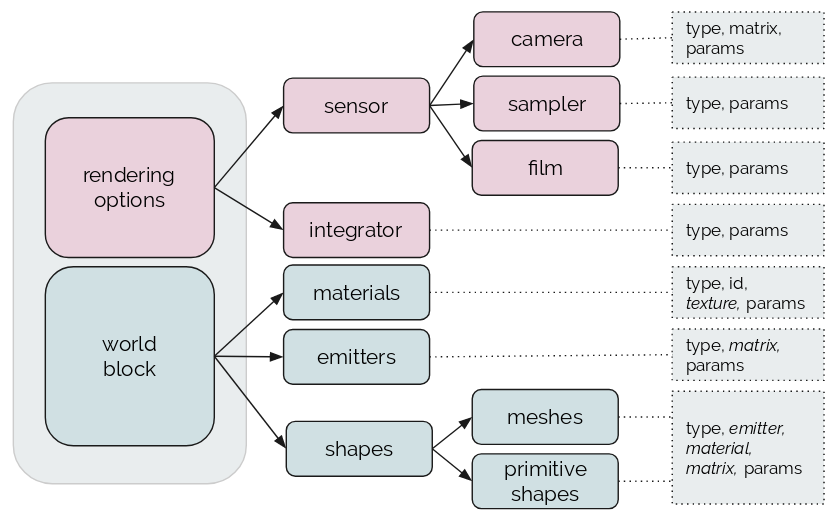
\includegraphics[width=\textwidth,height=\textheight,keepaspectratio]{images/4_system_architecture/canonicalrep.png}
  \caption{Structure of our canonical scene representation, consisting of rendering options and scene data. The attributes stored for each component are shown on the rectangles on the right.}
  \label{fig:canonicalrep}
\end{figure}

%\subsubsection{Scene-wide Rendering Options}
The \textit{Rendering Options}
%\noindent \textbf{Rendering Options}
specify the integration and sampling techniques used for
rendering, as well as camera and film properties. These include, for instance, camera position, camera matrix, image resolution, field of view, etc.
Table~\ref{tab:summary} summarizes all types, parameters, and additional attributes associated with each component of our canonical scene representation. 

%\subsubsection{World Block}
The \textit{World Block} describes the materials, global emitters, and shapes present in the scene.
%
A {\it material} (\eg, glass, plastic, metal, etc.) may have one or more associated textures. {\it Global emitters} represent all kinds of light sources, except area light sources, which are represented as shapes. These include conventional environment, spot, directional, and point light sources, as well more specific ones such as {\it sun} and {\it sky}.
%The \textbf{material} directive is represented in a structure with: a type \red{(examples of types?)}, an id, an optional texture and a list of parameters.
%
A {\it shape} can be a polygonal mesh or a geometric primitive such as a rectangle, disk, cube, or sphere, for instance. 
%an optional area emitter, an optional material reference, an optional transformation matrix and a list of parameters.

%The \textbf{texture} directive is represented in a structure with: a type, an id and a list of parameters. \red{[Where are the textures themselves stored?]}

%The \textbf{global emitter} directive is represented in a structure with: a type, an optional transformation matrix and a list of parameters.

\begin{center}
    \begin{tabular}{ l | l | l | l }
    \hline
    Directive 		& Type 				& Params 			& Others		\\ \hline
    integrator		& path tracer 			& max depth 			& -			\\
			& bidirectional path tracer 	& russian roulette depth	&			\\
			& metropolis light transport	& photon count			&			\\
			& photon mapping		& photon mapping lookup radius	&			\\
			& progressive photon mapping	& number of iterations		&			\\
			& direct lighting		& number of markov chains	&			\\ \hline
    sampler		& random			& samples per pixel		& -			\\
			& stratified			& scramble			&			\\
			& halton			&				&			\\
			& sobol				&				&			\\ \hline
    film		& ldr				& image width			& -			\\
			& hdr				& image height			&			\\
			&				& filter			&			\\
			&				& file extension (png, ...) 	&			\\ \hline
    camera		& perspective			& fov				& view matrix		\\
			& orthographic			& lens apperture		&			\\
			& environment			& focal distance		&			\\
			& realistic			& shutter open			&			\\
			&				& shutter close			&			\\
			&				& near clip			&			\\
			&				& far clip			&			\\ \hline
    materials		& metal				& kd				& texture (id, type, params)	\\ 
			& glass				& ks				&			\\
			& substrate/glossy		& transmittance			&			\\
			& matte/diffuse			& reflectance			&			\\
			& translucent			& roughness			&			\\
			& uber				& IOR				&			\\
			&				& eta				&			\\
			&				& k				&			\\
			& 				& id				&			\\
			& 				& ...				&			\\ \hline
    shapes		& mesh (ply/obj)		& filename			& model matrix		\\
			& cube				& center			& area emitter		\\
			& rectangle			& radius			& unnamed material	\\
			& sphere			& points			&			\\
			& disk				& normals			&			\\
			& trianglemesh			& uv mapping			&			\\
			& 				& ...				&			\\ \hline
    global emitters	& environment mapping		& radiance			& model matrix		\\
			& point				& filename			& 			\\
			& spot				& from (origin)			&			\\
			& sun				& to (direction)		&			\\
			& sky				& area (spot)			&			\\
			& directional			& ...				&			\\
			& distant			&				&			\\
    \end{tabular}
\end{center}
    

\section{The Export Module}

The export module is at the core of our system. While the import module deals with a single proprietary scene representation at a time, the export module has to map between materials and scene properties from two proprietary representations. 
In this case, there are several delicate cases to
consider. Matrix transformations, native shapes, environment mapping coordinates and, mostly, materials are
some of the components that vary greatly between renderers. 
In several situations, there is no direct mapping between them. Still, our system should provide an output representation that, once rendered with the target system, best approximates the results obtained by the source rendering system with the input scene description. 
Achieving such results required extensive experimentation with parameters of the various systems. Next, we discuss a few relevant aspects one should consider.    
  
%After the data is loaded into our canonical representation, it can be converted into any of the supported formats.
% \subsubsection{Converting Matrices}
%\noindent 
\subsection{Matrix Conversion}
There are several issues to consider when converting matrices between renderers.
%A few things we had to keep in mind were: 
Do the two renderers use different coordinate systems (either left-handed or right-handed)? 
%does this renderer use a left or right coordinate system? Does this renderer 
Do they represent matrices in the scene file using a direct representation or its
inverse-transpose? How is the object-world transformation represented for
shapes?

Mitsuba uses a right-hand coordinate system, while PBRT and LuxRender use a
left-hand one. This means that, when converting between Mitsuba and the other
two, one has to mirror the x-axis of all camera matrix transformations. This is
also the case for environment map positioning and object-world
transformations. Moreover, Mitsuba's scene files contain a world-to-camera transformation matrix (\ie, view matrix),
while PBRT and LuxRender scene files use the view matrix inverse transpose.

%\green{Furthermore, Mitsuba scene files have their camera position specified as a 
%world-to-camera transformation matrix, while PBRT and LuxRender scene files have 
%theirs as a camera-to-world transformation matrix. Therefore, converting the 
%camera positioning between Mitsuba and the other two renderers means we have to 
%compute the inverse transpose of this transformation matrix.}

% \red{Mitsuba also has its camera transformation matrix specified as a camera-to-world
%  transformation, while PBRT and LuxRender do not. Therefore, when converting the
% camera look-at matrix between these renderers, we had to compute the inverse
% transpose of the specified matrix. }

% \subsubsection{Converting Materials}
\subsection{Material Conversion}
Materials are the most delicate aspect of scene conversion. Materials have
spectral and roughness properties that absolutely must be correctly mapped. 
However, most renderers have very different implementations
for common subsurface scattering models (BSDFs), making it hard to
predict the mapping between the parameters of two such implementations.

Mitsuba uses a more physics-oriented approach: a material can be diffuse,
conductor, dielectric, plastic, translucent, or a bumpmap.
It also has other types of materials, but those are not supported in the current implementation of our system.
The material type in Mitsuba changes as the material contains any form of
surface roughness, becoming a ``rough'' version of itself (for instance, a rough
metal becomes a roughconductor).
%
PBRT and LuxRender materials have roughness parameters, making it unnecessary to
change the material's name.

%The major problem was faced when converting metals from and to LuxRender. 
To represent the material's reflectance, PBRT and Mitsuba use one index of refraction ($\eta$) and one absorption 
coefficient (\textit{k}) per color channel. 
LuxRender, however, uses a so-called ``{\it Fresnel texture}'', specifying a 
single value of $\eta$ and \textit{k} for all channels. Alternatively, LuxRender allows the specification of a single RGB 
color value for the material's reflectance. Therefore, correctly converting metal colors between LuxRender and PBRT or Mitsuba is not well defined, 
and is not supported in the current implementation of our system.

\subsection{Shape Conversion}
Shape directives can be split into two categories: {\it primitive shapes}, which can
be used to specify primitives such as {\it rectangles, disks, cubes}, and {\it spheres};
and {\it 3D meshes}, which are stored in external files. 
%
Converting primitive shapes requires more attention than converting external 3D meshes. 
Mitsuba has directives for rectangle, disk, cube and sphere, while PBRT and LuxRender do not. 
Mitsuba's primitives are defined by some parameters (\eg, vertex positions, radius) which can be modified by 
a transformation (model) matrix. To reproduce these primitives in PBRT and 
LuxRender, an {\it internal triangle mesh} must be used. This is done by specifying the position, normal, and texture coordinates for each vertex in the mesh representing a given primitive. One should note that these internal meshes do not use the same representation as the 3D meshes stored in files.

Converting PBRT and LuxRender internal triangle meshes into Mitsuba primitive shapes is a more involving process. Since Mitsuba's 
primitives have predefined coordinates, converting vertices from PBRT or LuxRender internal meshes into 
these coordinates requires obtaining the transformation matrix that maps PBRT or LuxRender vertices 
to Mitsuba's predefined points. Our system takes care of this automatically.

Converting external 3D meshes is simple, as all rendering systems have directives
for this purpose. PBRT, however, does not support Object File Wavefront 3D
(.obj) files. 
%the user with mesh converting tools.
In this case, our system issues a warning, making the user aware of the need to convert .obj files off-line.

% Since the triangle mesh directive specifies each points in world coordinates, 
% The reverse process, however, is more complicated. The triangle mesh directive
% specifies the coordinates, normal and uv mapping for the points forming a
% triangle. In order to recover a transformation matrix for the corresponding
% Mitsuba primitive, \red{these points have to be multiplied by the original Mitsuba
% canonical coordinates in the correct order.}

\subsection{Global Emitter Conversion}
Global emitters can be used to emulate environment lighting, such as the sun, the
sky, or an environment map. Converting global emitters can be tricky, mainly
because different rendering systems do not implement the same algorithms and directives. 
For instance, Mitsuba and LuxRender implement {\it sun} and {\it sky} directives, while PBRT does not.
%However, these directives can be converted from Mitsuba and LuxRender to PBRT. 
A sun directive can be simulated in PBRT using a distant light. A sky directive can
be simulated using an environment map of a clear sky.
While PBRT and LuxRender access environment maps using spherical coordinates, 
Mitsuba uses a latitude-longitude format. Thus, a conversion between the two representations is required. 
  
%
Converting a PBRT distant light into
a sun directive for Mitsuba or LuxRender is straightforward. However, converting a PBRT
environment map into a sky directive lends to an ambiguous situation, as the converter would require additional information to decide 
whether the environment map should be treated as a regular environment map, or as a sky directive.
Our system solves this ambiguity by asking the user if the environment map should be converted to a sky
emitter.

Another sensitive point to consider is converting environment mapping indexation. 
PBRT and LuxRender access environment maps using spherical coordinates, 
($\theta$, $\phi$), 
while Mitsuba uses a latitude-longitude format.   
% (\textit{x}, \textit{y} and \textit{z}).
% , as  shown in Figure \ref{fig:mitdocemitter}. 
A conversion between the two representations is required. 
% can be done by applying a \red{transformation matrix on the 
% environment map, rotating the \textit{x}, \textit{y} and \textit{z} axes to match the differing axis setup.} 

\begin{figure}[h]
  \centering
  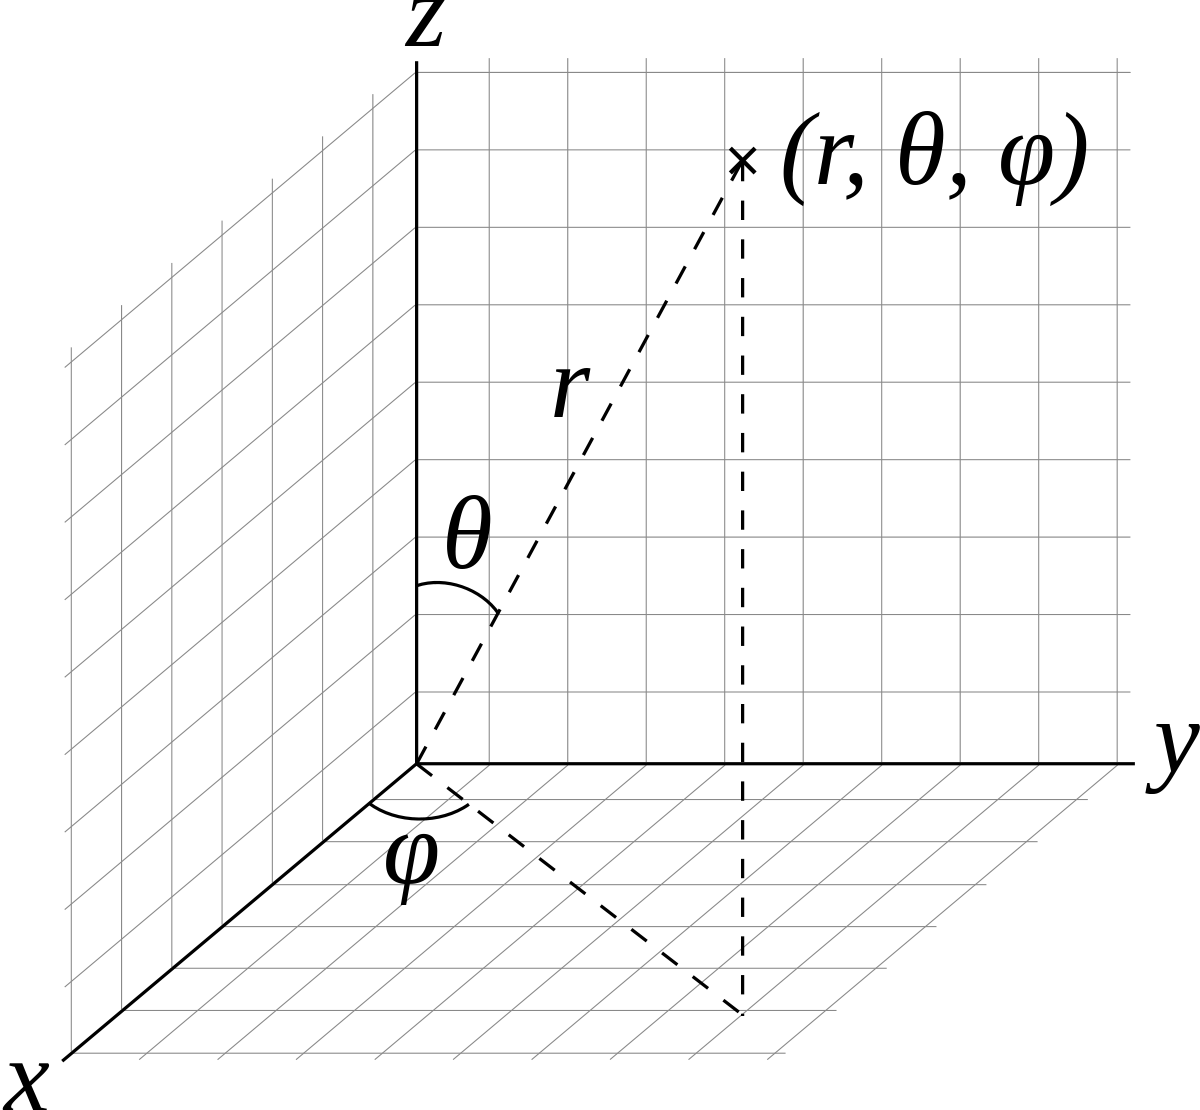
\includegraphics[width=0.4\textwidth,height=\textheight,keepaspectratio]{images/4_system_architecture/spherical_coordinates.png}
  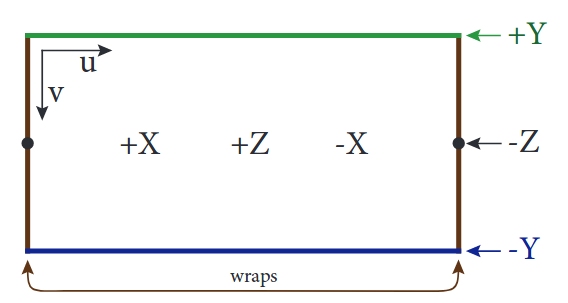
\includegraphics[width=0.4\textwidth,height=\textheight,keepaspectratio]{images/4_system_architecture/mitdocemitter.png}
  \caption{Illustration of the coordinate conventions used by PBRT and LuxRender 
  (left) and by Mitsuba (right) for indexing environment map uv coordinates.}
  \label{fig:mitdocemitter}
\end{figure}



\chapter{Results}
\label{sec:results}

%This chapter discusses results and limitations of our system.

Our system is available on-line~\cite{sceneConverter}.
We have tested it on a large number of scenes, including the 32 scenes available
at Bitterli's rendering resources website~\cite{resources16}. 
%We validated our system's conversion using scenes from Bitterli's 32 resources 
%\cite{resources16}. 
Here, we include a few examples to illustrate its results on scenes that explore different 
types of materials, 3D meshes and primitive shapes, image and 
procedural textures, and various lighting styles. They include most elements typically found in scenes used by physically-based rendering systems.  The time required to convert a scene is about 0.5 seconds on a typical PC (Intel i5 3.8 GHz).
% 
%We chose scenes that provided a wide variety of directives 
%in order to cover most commonly used directives. These scenes include: different 
%types of materials and bump maps; 3D meshes and primitive shapes; image and 
%primitive textures; area and environment lighting. 
%
The scenes were rendered using Mitsuba 0.5.0, PBRT v3, and LuxRender v1.6 on 
Ubuntu 14.04 LTS. All scenes were rendered using between 5,000 and 8,000 samples per pixel (spp). For any given scene,
the same number of samples per pixel was used with all rendering systems. 

Figure~\ref{fig:teaser} shows a coffee maker containing various materials, including glass, plastic, and metal, as well as textures. The input scene description was provided in the format for PBRT v3, whose rendering is shown on the left. The images at the center and on the right were produced by Mitusuba and LuxRender, respectively, from scene representations automatically converted by our system. 
%from the input scene file. 
Note how the object details have been faithfully preserved in these renderings.

The \textit{Wooden Staircase} scene (Figure~\ref{fig:staircase}) contains many geometric objects and textures. 
A LuxRender scene description was provided as input and its rendering is shown in (a). The images shown in (b) and (c) were produced 
by PBRT v3 and Mitsuba, respectively, from scene representations automatically converted by our system. 

The \textit{Teapot} scene (Figure \ref{fig:teapot}) contains a shiny object, environment lighting, and a procedural texture. The input scene description was also provided in the LuxRender format. Figures~\ref{teatpot_PBRT} and \ref{teapot_Mitsuba} show the renderings produced by PBRT v3 and Mitsuba, respectively, from scene descriptions converted by our system.

Figure~\ref{fig:bidir-cornell} shows two scenes, \textit{Veach Bidir Room} and \textit{Cornell Box}. The first includes caustics, while the second only contains diffuse surfaces. A Mitsuba scene description was provided as input for each of these scenes, whose renderings are shown on the first column of Figure~\ref{fig:bidir-cornell}. Columns (b) and (c) show, respectively, the renderings produced by PBRT v3 and LuxRender using scene descriptions converted by our system.    

\begin{figure*}[h!t]
	\centering
	
	\subfloat[LuxRender]{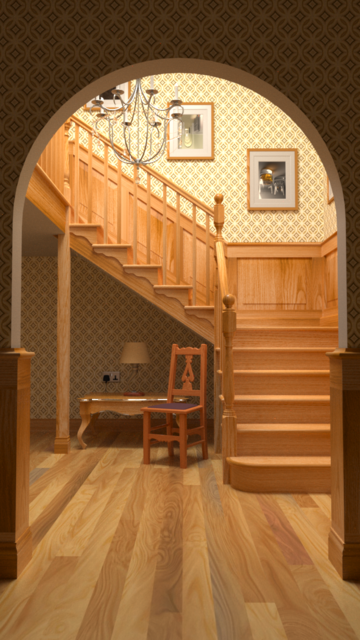
\includegraphics[width=0.32\linewidth]{images/5_results/staircase/1_from_lux.png}
		\label{staircase_Lux}
	}
	\subfloat[PBRT v3]{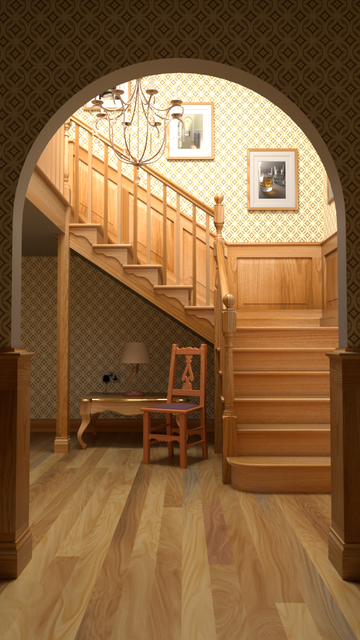
\includegraphics[width=0.32\linewidth]{images/5_results/staircase/3_to_pbrt.png}
		\label{staircase_PBRT}
	}
	\subfloat[Mitsuba]{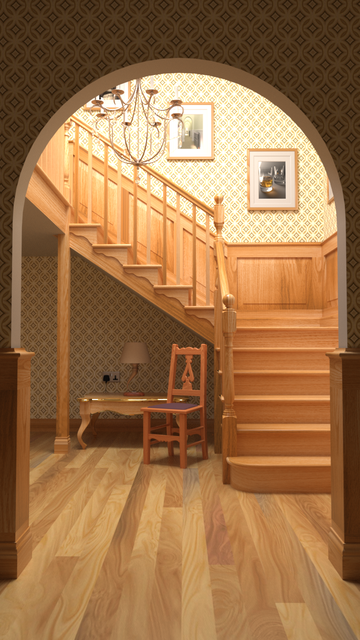
\includegraphics[width=0.32\linewidth]{images/5_results/staircase/2_to_mitsuba.png}
		\label{staircase_Mitsuba}
	}
	\caption{\textit{The Wooden Staircase} scene. Input scene description for LuxRender (a).
		Renderings produced by PBRT v3 (b) and Mitsuba (c),
		from scene descriptions converted by our system. }
	\label{fig:staircase}
\end{figure*}

\begin{figure*}
  \centering
  \subfloat[LuxRender]{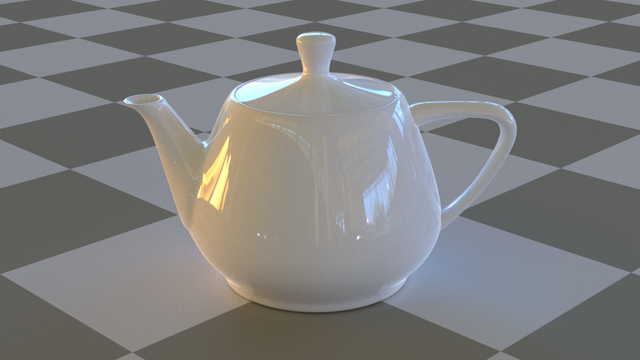
\includegraphics[width=0.32\linewidth]{images/5_results/teapot/1_from_lux.png}\label{teapot_Lux}}
  \subfloat[PBRT v3]{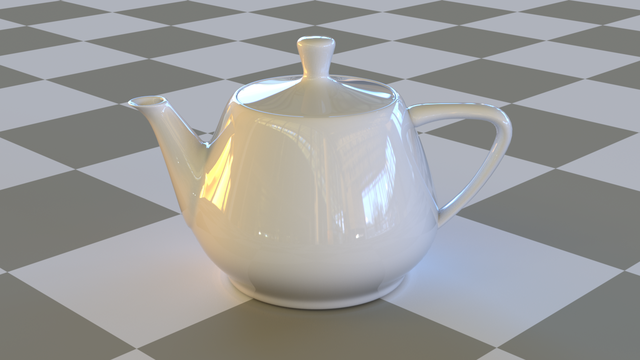
\includegraphics[width=0.32\linewidth]{images/5_results/teapot/3_to_pbrt.png}\label{teatpot_PBRT}}
  \subfloat[Mitsuba]{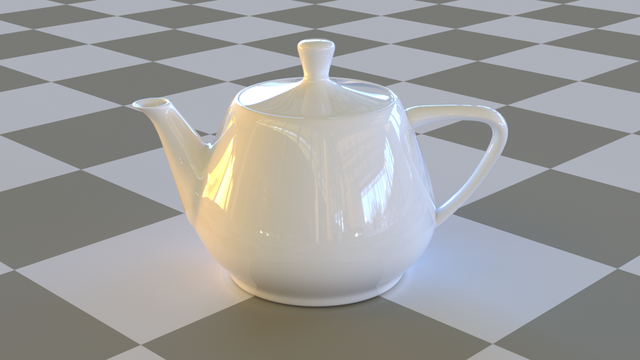
\includegraphics[width=0.32\linewidth]{images/5_results/teapot/2_to_mitsuba.png}\label{teapot_Mitsuba}}
  \caption{\textit{Teapot} scene. Input scene description for LuxRender (a). Renderings produced by PBRT v3 (b) and Mitsuba (c), from scene descriptions converted by our system.}
  \label{fig:teapot}
\end{figure*}

\begin{figure*}
\centering
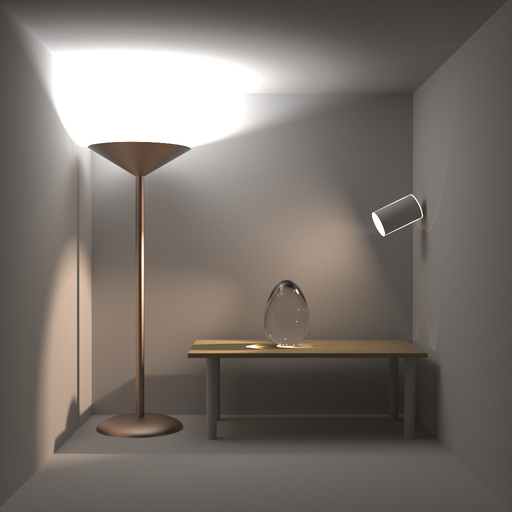
\includegraphics[width=0.32\linewidth]{images/5_results/veach-bidir/1_from_mitsuba.png}
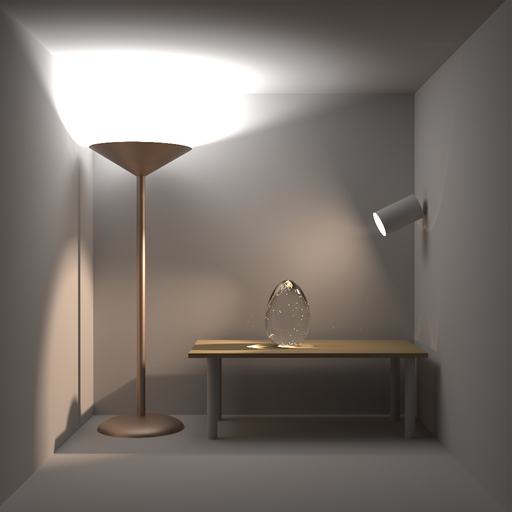
\includegraphics[width=0.32\linewidth]{images/5_results/veach-bidir/2_to_pbrt.png}
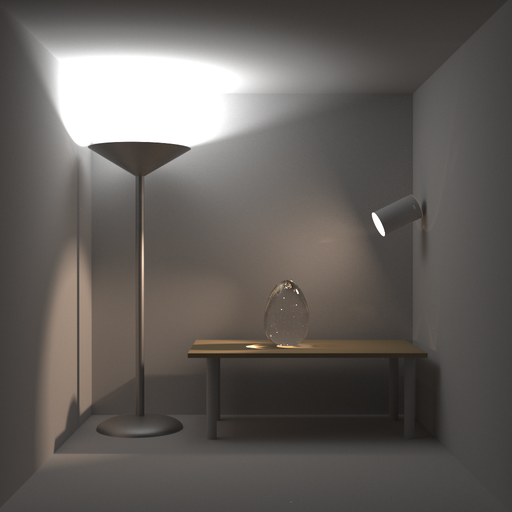
\includegraphics[width=0.32\linewidth]{images/5_results/veach-bidir/3_to_lux.png}
%\vspace{-0.2cm}
\subfloat[Mitsuba]{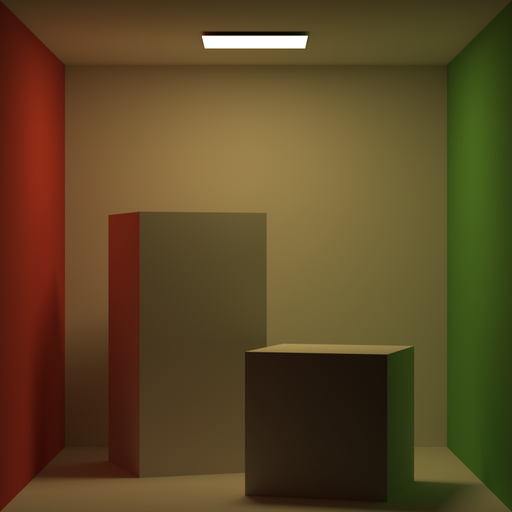
\includegraphics[width=0.32\linewidth]{images/5_results/cornell-box/1_from_mitsuba.png}
}	
\subfloat[PBRT v3]{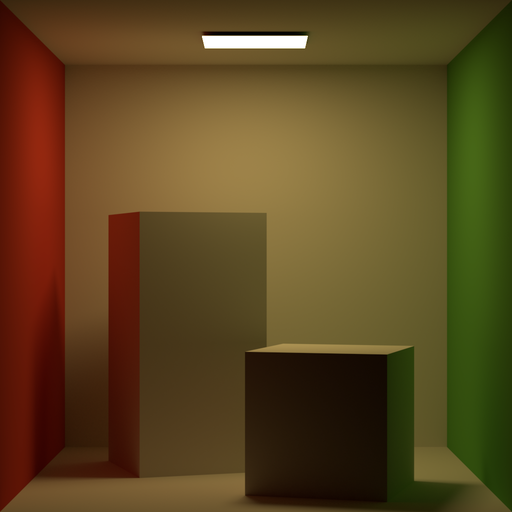
\includegraphics[width=0.32\linewidth]{images/5_results/cornell-box/2_to_pbrt.png}
}	
\subfloat[LuxRender]{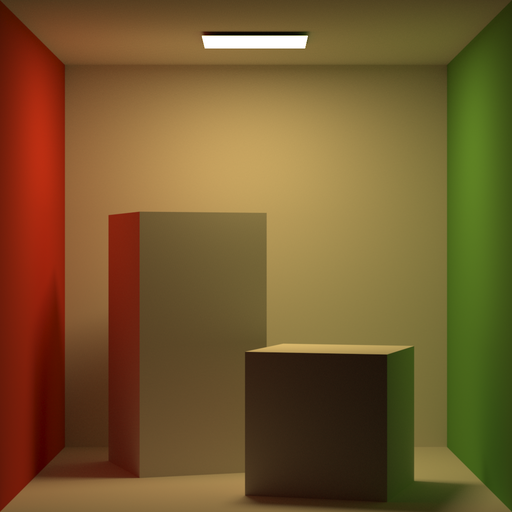
\includegraphics[width=0.32\linewidth]{images/5_results/cornell-box/3_to_lux.png}}
\caption{\textit{Veach, Bidir Room} (top) and \textit{Cornell Box} (bottom). Input scene descriptions for 
 Mitsuba (a). Renderings produced by PBRT v3 (b) and LuxRender (c),
 from scene descriptions converted by our system.}
\label{fig:bidir-cornell}
\end{figure*}

\section{Discussion}

The renderings produced by different rendering systems may exhibit significant differences in color or shading due to features unsupported by some renderers.  
For instance, consider the use of a light source to emulate the sun. In PBRT and LuxRender, this directive is implemented as a distant white light.
Mitsuba, in turn, emulates the sun using a distant environment light implemented according to a technique 
described in \cite{Preetham}, which produces a warm-colored, distant light source. Thus, when the sun directive is used, Mitsuba renderings present a different color compared to the other two. This situation is illustrated in Figure~\ref{fig:dining-room}.

LuxRender does not properly handles a combination of sun directive and local light sources. This is illustrated in Figure~\ref{lamp_Lux}, where hard shadows have turned soft. The difference in colors are due to the sun directive, as discussed above.

The supplemental materials included with this submission show all the examples presented in the paper plus additional ones. We would like to encourage the reader to explore them, where one can inspect the images at their original resolutions.

\section{Limitations}
%In order to minimize scope issues, we restricted the number of directives interpreted by our system. 
Scene-description directives found in one rendering system but without correspondence in the other two renderers are not handled by our system. That is the case, for instance, of Mitsuba-only materials like \textit{phong} and \textit{blendbsdf}. 

The current version of our system does not support the conversion of hair or participating media. 
%We also did not convert the color for metal 
%materials in LuxRender given the issues discussed in \ref{systemarch}. The 
%latter can be observed in Figure \ref{fig:veach-bidir} - we can see the lack of a 
%copper color on the lamp in the image rendered by LuxRender.
%
As discussed in Section~\ref{sec:systemarch}, LuxRender treats material reflectance differently from PBRT and Mitsuba. Thus, properly converting metal colors to LuxRender is a challenging task, not currently supported by our system. This is illustrated in Figure~\ref{fig:MIS}, where the rendering of metal obtained from a scene converted to and rendered with LuxRender looks darker.  

\begin{figure*}
  \centering
  \subfloat[LuxRender]{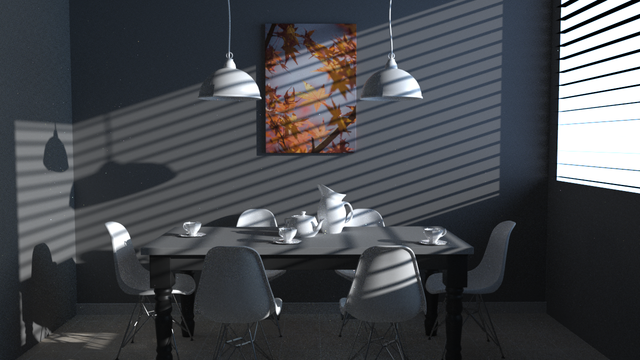
\includegraphics[width=0.5\linewidth]{images/5_results/dining_room/1_from_lux.png}\label{breakfast_Lux}}\\
  \subfloat[PBRT v3]{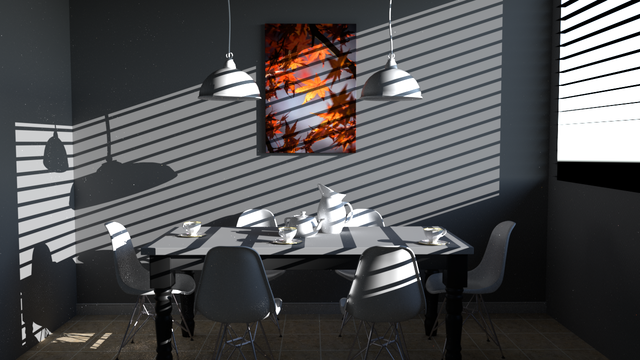
\includegraphics[width=0.5\linewidth]{images/5_results/dining_room/3_to_pbrt.png}\label{breakfast_PBRT}}\\
  \subfloat[Mitsuba]{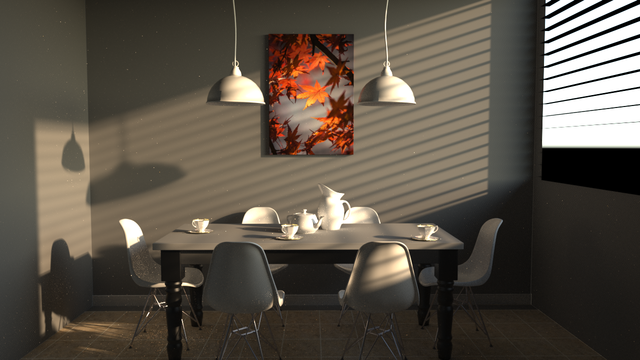
\includegraphics[width=0.5\linewidth]{images/5_results/dining_room/2_to_mitsuba.png}\label{breakfast_Mitsuba}}
  \caption{\textit{The Breakfast Room} scene. Input scene description for LuxRender (a). Renderings produced by PBRT v3 (b) and Mitsuba (c), from scene descriptions converted by our system. Mitsuba's sun directive produces a warm-colored lighting.}
  \label{fig:dining-room}
\end{figure*}

\begin{figure}
  \centering
  \subfloat[Mitsuba]{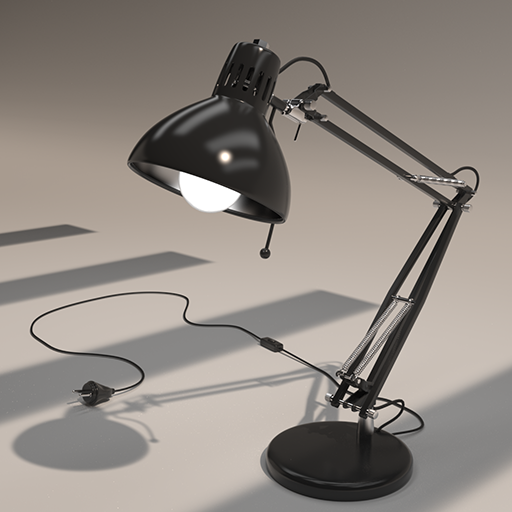
\includegraphics[width=0.32\linewidth]{images/5_results/lamp/1_from_mitsuba_s.png}\label{lamp_Mitsuba}}
  \subfloat[PBRT v3]{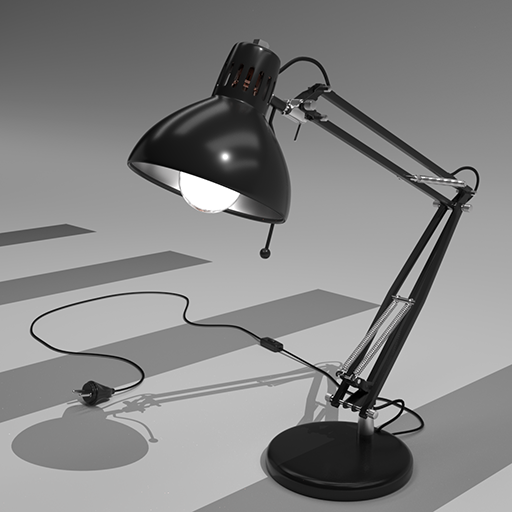
\includegraphics[width=0.32\linewidth]{images/5_results/lamp/2_to_pbrt_s.png}\label{lamp_PBRT}}
  \subfloat[LuxRender]{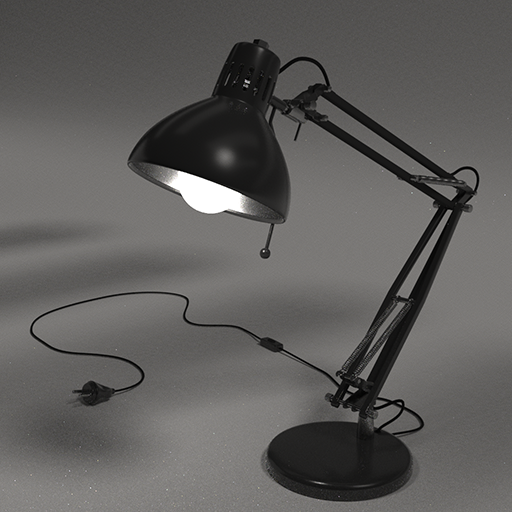
\includegraphics[width=0.32\linewidth]{images/5_results/lamp/3_to_lux_s.png}\label{lamp_Lux}}
  \caption{\textit{Little Lamp} scene. Input scene description for Mitsuba (a). Renderings produced by PBRT v3 (b) and LuxRender (c), from scene descriptions converted by our system.}
  \label{fig:lamp}
\end{figure}

\begin{figure}
  \centering
  \subfloat[PBRT v3]{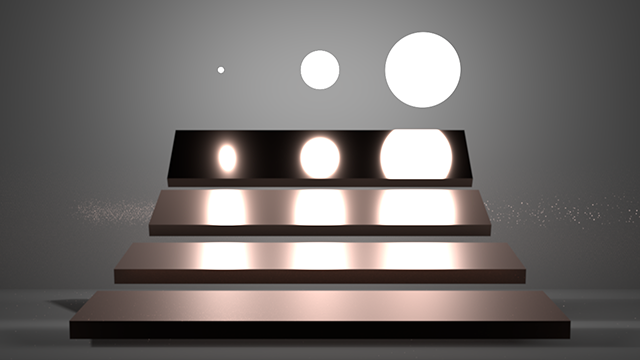
\includegraphics[width=0.6\linewidth]{images/5_results/veach-mis/1_from_pbrt_s.png} \label{MIS_PBRT}}\\
  \subfloat[Mitsuba]{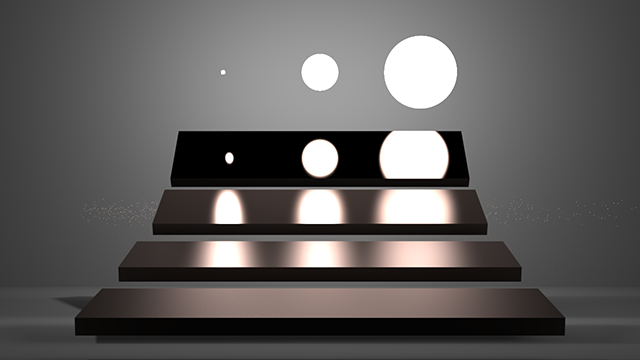
\includegraphics[width=0.6\linewidth]{images/5_results/veach-mis/2_to_mitsuba_s.png}\label{MIS_Mitsuba}}\\
  \subfloat[LuxRender]{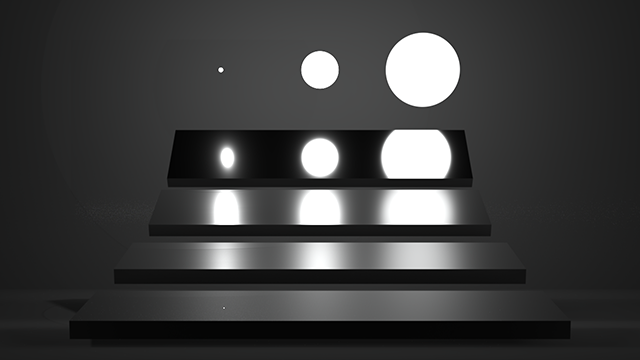
\includegraphics[width=0.6\linewidth]{images/5_results/veach-mis/3_to_lux_s.png}\label{MIS_Lux}}
  \caption{\textit{Veach, MIS}. Renderings by PBRT v3 (a), Mitsuba (b), and LuxRender (c). Converting metal colors to LuxRender is a challenging task, not currently supported by our system.} 
  \label{fig:MIS}
\end{figure}

%\begin{figure}
%\centering
%\subfloat[PBRT v3]{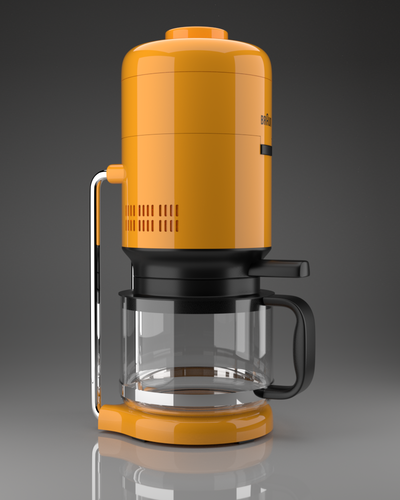
\includegraphics[width=0.32\linewidth]{figs/4_results/glass_of_water/1_from_pbrt.png}
%	\label{glass_PBRT}		
%}	
%\subfloat[LuxRender]{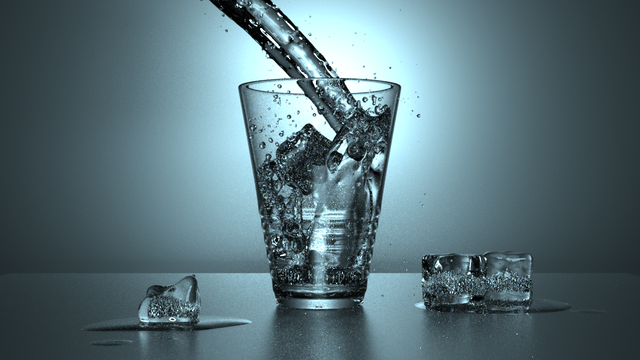
\includegraphics[width=0.32\linewidth]{figs/4_results/glass_of_water/2_to_lux.png}
%	\label{glass_Lux}		
%}	
%\subfloat[Mitsuba]{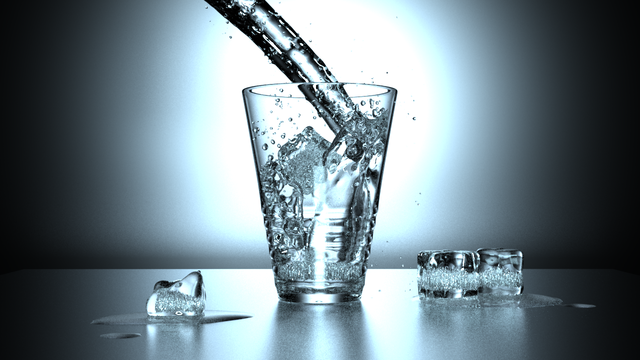
\includegraphics[width=0.32\linewidth]{figs/4_results/glass_of_water/3_to_mitsuba.png}
%	\label{glass_Mitsuba}		
%}	
%\caption{\textit{Glass of Water}. Input scene description for PBRT v3 (a).
%	Renderings produced by LuxRender (b) and Mitsuba (c),
%	from scene descriptions converted by our system. } 
%\label{fig:glass-of-water}
%\end{figure}






\chapter{Conclusion}
\label{sec:conclusion}
We presented a system for automatic conversion among scene file formats used by Monte Carlo physically-based rendering systems. 
It enables algorithms implemented using different renderers to be tested on similar scene descriptions, providing better means of assessing the strengths and limitations of MC rendering techniques. 
%
Our system can be easily integrated with the API recently introduced by~\cite{Santos:2018:FBKSD}, allowing researchers and developers to exploit full orthogonality among MC algorithms, rendering systems, and scene files.   

We have demonstrated the effectiveness of our system by converting scene description among three of the most popular MC rendering systems: PBRT v3, Mitsuba, and LuxRender. Providing support to additional renderers only requires specializing the import and export modules described in Section~\ref{sec:systemarch} for the given renderers. Our system is freely available and we encourage developers to provide support for other renderers.  

In the future, we would like to add support for the conversion of hair and participating media, as well as for other rendering systems.
By documenting limitations and incompatibilities found among different renderers, our work might stimulate efforts to reduce these differences.   


% referências
% aqui será usado o environment padrao `thebibliography'; porém, sugere-se
% seriamente o uso de BibTeX e do estilo abnt.bst (veja na página do
% UTUG)

\bibliographystyle{abntex2-alf}
\bibliography{biblio}

\end{document}
